\makeatletter

\long\gdef\versochapter#1{
  \vspace*{3cm}
  \minipage{\textwidth}
  \hfill\includegraphics[width=0.5\textwidth]{\chapterimage@cx}\par
  \vspace*{6pt}
  \hfill\minipage{0.75\textwidth}
  {\HUGE\bfseries\flushright #1\endflushright}
  \endminipage
  \endminipage
  \newpage


\vspace*{10cm}
\@specialfalse
\@openleftfalse
\@openanyfalse
\@openrighttrue
}


\newgeometry{bottom=2.5cm}

\cxset{
   chapter image/.code={\def\chapterimage@cx{#1}},
   chapter opening/.is choice,
   chapter opening/verso/.code={\@specialtrue\@openlefttrue
   \gdef\customdesign@cx##1{\versochapter{##1}}}
}

\cxset{
 custom=versochapter,
 chapter image={vespa.jpg},
 chapter opening=verso,
 name={},
 numbering=none,
 number font-size=LARGE,
 number font-family=rmfamily,
 number font-weight=bfseries,
 number before=,
 number dot={},
 number after=,
 number position=leftname,
 chapter font-family=sffamily,
 chapter font-weight=\normalfont,
 chapter font-size=\Large,
 chapter before={\vspace*{0pt}\par},
 chapter after={\hfill\hfill\par},
 chapter color={black!90},
 number color=purple,
 title beforeskip={\vspace*{0pt}},
 title afterskip={\vspace*{0.4\textheight}\par},
 title before={},
 title after={},
 title font-family=sffamily,
 title font-color=purple,
 title font-weight=bfseries,
 title font-size=LARGE,
 header style=plain,
 pagestyle=plain,
 }

\makeatletter
\@specialtrue
\makeatother



\chapter{Verso Chapters}

\parindent1.5em

{\Huge T}he theme of this template is from a book called 
{ \textit{From Western attitudes toward death from the middle ages to the present}, Philippe Ari\'es. London, 1974.

\begin{figure}
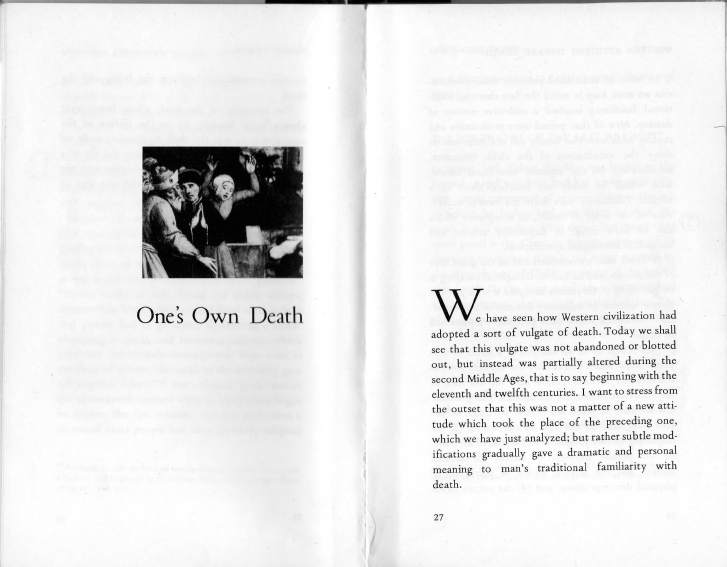
\includegraphics[width=\textwidth]{./chapters/versochapter01.png}
\caption{Chapter opening on verso page.}
\end{figure}

I will quote Oliver Sacks words verbatim, as I cannot ever imagine that I can do it better:

\begin{quote}
A MONTH ago, I felt that I was in good health, even robust health. At 81, I still swim a mile a day. But my luck has run out — a few weeks ago I learned that I have multiple metastases in the liver. Nine years ago it was discovered that I had a rare tumor of the eye, an ocular melanoma. Although the radiation and lasering to remove the tumor ultimately left me blind in that eye, only in very rare cases do such tumors metastasize. I am among the unlucky 2 percent.

I feel grateful that I have been granted nine years of good health and productivity since the original diagnosis, but now I am face to face with dying. The cancer occupies a third of my liver, and though its advance may be slowed, this particular sort of cancer cannot be halted.

It is up to me now to choose how to live out the months that remain to me. I have to live in the richest, deepest, most productive way I can. In this I am encouraged by the words of one of my favorite philosophers, David Hume, who, upon learning that he was mortally ill at age 65, wrote a short autobiography in a single day in April of 1776. He titled it “My Own Life.”

“I now reckon upon a speedy dissolution,” he wrote. “I have suffered very little pain from my disorder; and what is more strange, have, notwithstanding the great decline of my person, never suffered a moment’s abatement of my spirits. I possess the same ardour as ever in study, and the same gaiety in company.”

I have been lucky enough to live past 80, and the 15 years allotted to me beyond Hume’s three score and five have been equally rich in work and love. In that time, I have published five books and completed an autobiography (rather longer than Hume’s few pages) to be published this spring; I have several other books nearly finished.

Hume continued, “I am ... a man of mild dispositions, of command of temper, of an open, social, and cheerful humour, capable of attachment, but little susceptible of enmity, and of great moderation in all my passions.”

Here I depart from Hume. While I have enjoyed loving relationships and friendships and have no real enmities, I cannot say (nor would anyone who knows me say) that I am a man of mild dispositions. On the contrary, I am a man of vehement disposition, with violent enthusiasms, and extreme immoderation in all my passions.

And yet, one line from Hume’s essay strikes me as especially true: “It is difficult,” he wrote, “to be more detached from life than I am at present.”

Over the last few days, I have been able to see my life as from a great altitude, as a sort of landscape, and with a deepening sense of the connection of all its parts. This does not mean I am finished with life.

On the contrary, I feel intensely alive, and I want and hope in the time that remains to deepen my friendships, to say farewell to those I love, to write more, to travel if I have the strength, to achieve new levels of understanding and insight.\footnote{Oliver Sacks, a professor of neurology at the New York University School of Medicine, is the author of many books, including “Awakenings” and “The Man Who Mistook His Wife for a Hat.”}
\end{quote}

\begin{quote}
I have been increasingly conscious, for the last 10 years or so, of deaths among my contemporaries. My generation is on the way out, and each death I have felt as an abruption, a tearing away of part of myself. There will be no one like us when we are gone, but then there is no one like anyone else, ever. When people die, they cannot be replaced. They leave holes that cannot be filled, for it is the fate — the genetic and neural fate — of every human being to be a unique individual, to find his own path, to live his own life, to die his own death.

I cannot pretend I am without fear. But my predominant feeling is one of gratitude. I have loved and been loved; I have been given much and I have given something in return; I have read and traveled and thought and written. I have had an intercourse with the world, the special intercourse of writers and readers.

Above all, I have been a sentient being, a thinking animal, on this beautiful planet, and that in itself has been an enormous privilege and adventure.
\end{quote}

To load the template just type:

\begin{verbatim}
\cxset{%
 custom=versochapter,
 chapter image=vespa.jpg,
 chapter opening=verso}
\end{verbatim}





\makeatletter
\@specialfalse
\makeatother
